\renewcommand{\theequation}{\theenumi}
\begin{enumerate}[label=\thesubsection.\arabic*.,ref=\thesubsection.\theenumi]
\numberwithin{equation}{enumi}

\item \solution $p\brak{x, y} = Ax^2 + Bxy + Cy^2 + Dx + Ey + F$ can be represented as follow in the vector form:
\begin{align}
\vec{x}^T 
\myvec{
A & \frac{B}{2} \\
\frac{B}{2} & C
}
\vec{x} + 
\myvec{
D & E 
}
\vec{x} + F = 0
\end{align}

\item \begin{flushleft}
The given equation can be represented as follows in the vector form:
\end{flushleft}
\begin{align}
\vec{x}^T 
\myvec{
1 & 0 \\
0 & 0
}
\vec{x} + 
\myvec{
-2 & 0 
}
\vec{x} + 0 = 0 \label{eq:conics_main}
\end{align}

\item To find the roots $y=0$:
\begin{align}
x^2 - 2x &= 0 \\
x\brak{x-2} &= 0 \\
x &= 0,2
\end{align}

\item To verify:
\begin{enumerate}
\item Substitute $\vec{x} = \myvec{0\\0}$ in \eqref{eq:conics_main}
\begin{align}
\myvec{0\\0}^T 
\myvec{
1 & 0 \\
0 & 0
}
\myvec{0\\0} &+ 
\myvec{
-2 & 0 
}
\myvec{0\\0} + 0 \\
&\implies 0
\end{align}

\item  Substitute $\vec{x} = \myvec{2\\0}$ in \eqref{eq:conics_main}
\begin{align}
\myvec{2\\0}^T 
\myvec{
1 & 0 \\
0 & 0
}
\myvec{2\\0} &+ 
\myvec{
-2 & 0 
}
\myvec{2\\0} + 0 \\
&\implies 0
\end{align}
\end{enumerate}

\item \begin{figure}[!ht]
\centering
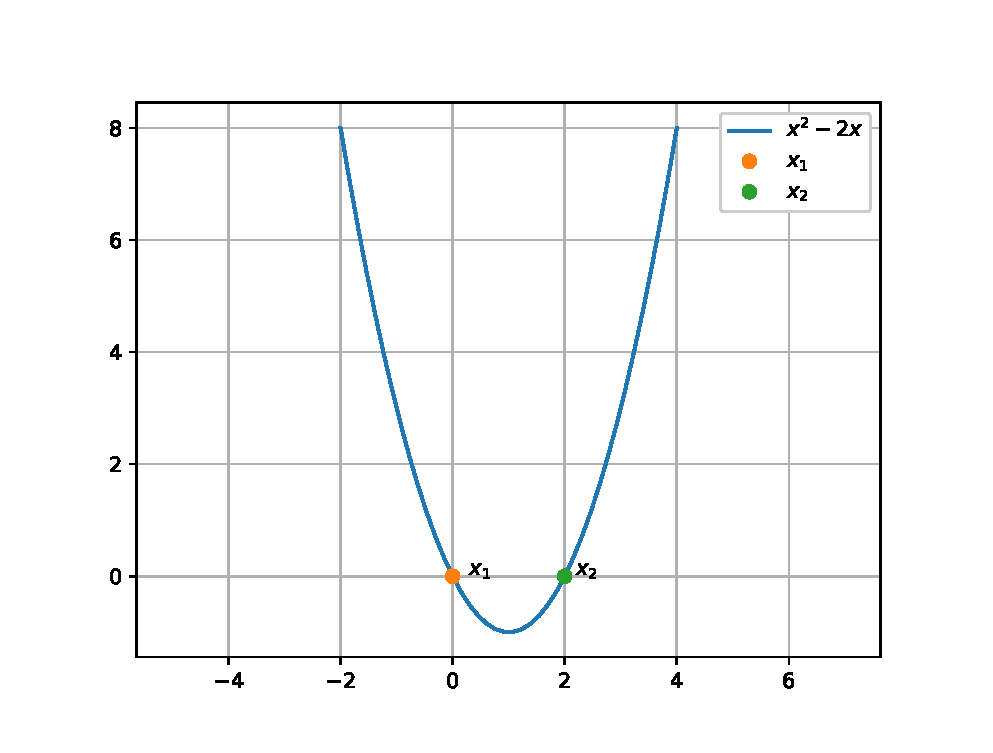
\includegraphics[width=\columnwidth]{./figs/conics_example/quadratic_equation.eps}
\caption{$x^2 -2x$ generated using python}
\label{fig:quadeq_conics_example}
\end{figure} 
The  following Python code generates Fig. \ref{fig:quadeq_conics_example}

\begin{lstlisting}
codes/conics_example/conics.py
\end{lstlisting}
\end{enumerate}